\section{Alternate protocol 2: General Search
Box}\label{alternate-protocol-2-general-search-box}

A general search text box is available to explore the manually curated
information in the ELM DB. This is a ``Full-text'' search which is
performed on selected columns of the database therefore some attention
(better term?) should be applied when evaluating the retrieved results.

\begin{figure}[h!]
\centering
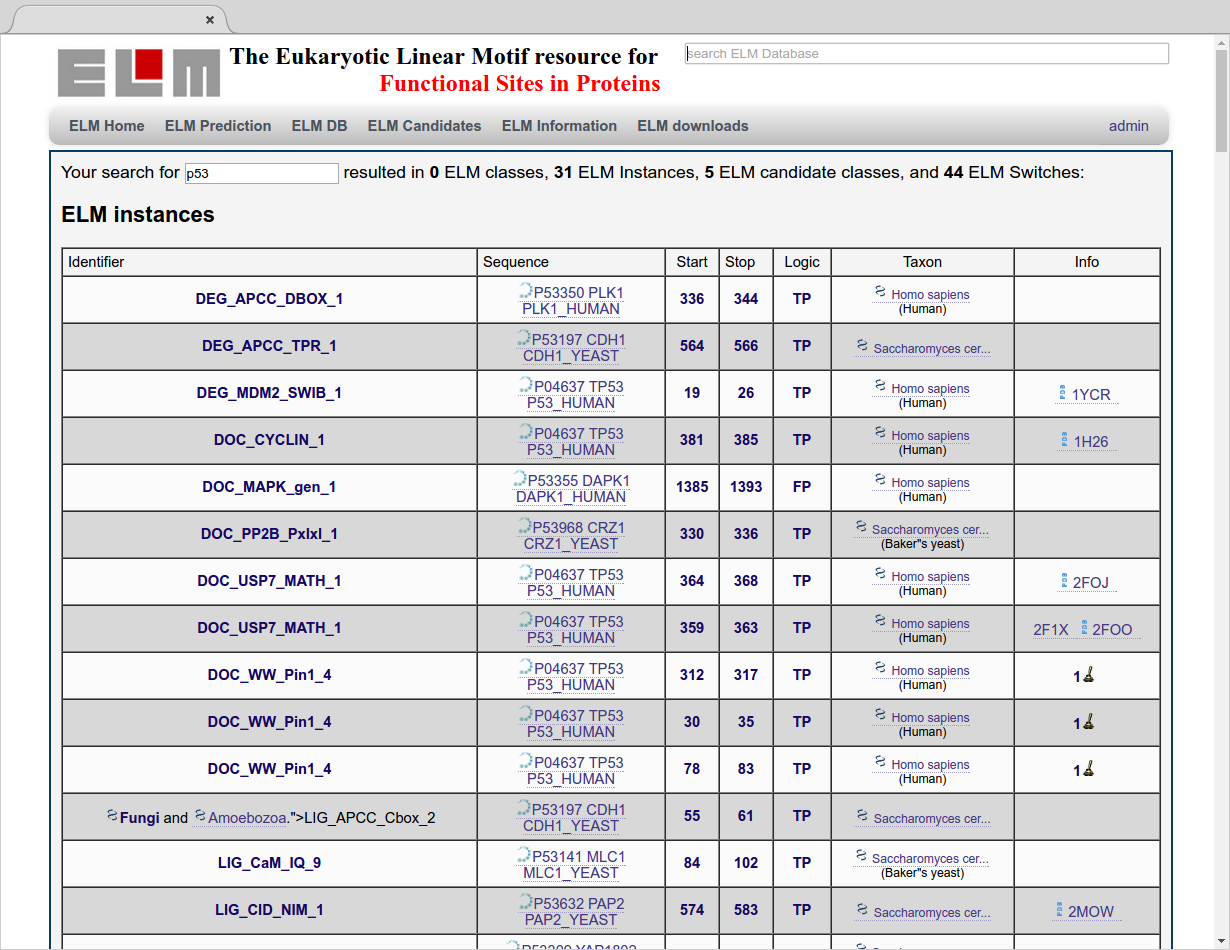
\includegraphics[width=\textwidth]{Figures/TP53_3/TP53_instances.png} 
\caption{\textbf{Figure TP53-AP1-1}}
\end{figure}

\begin{figure}[h!]
\centering
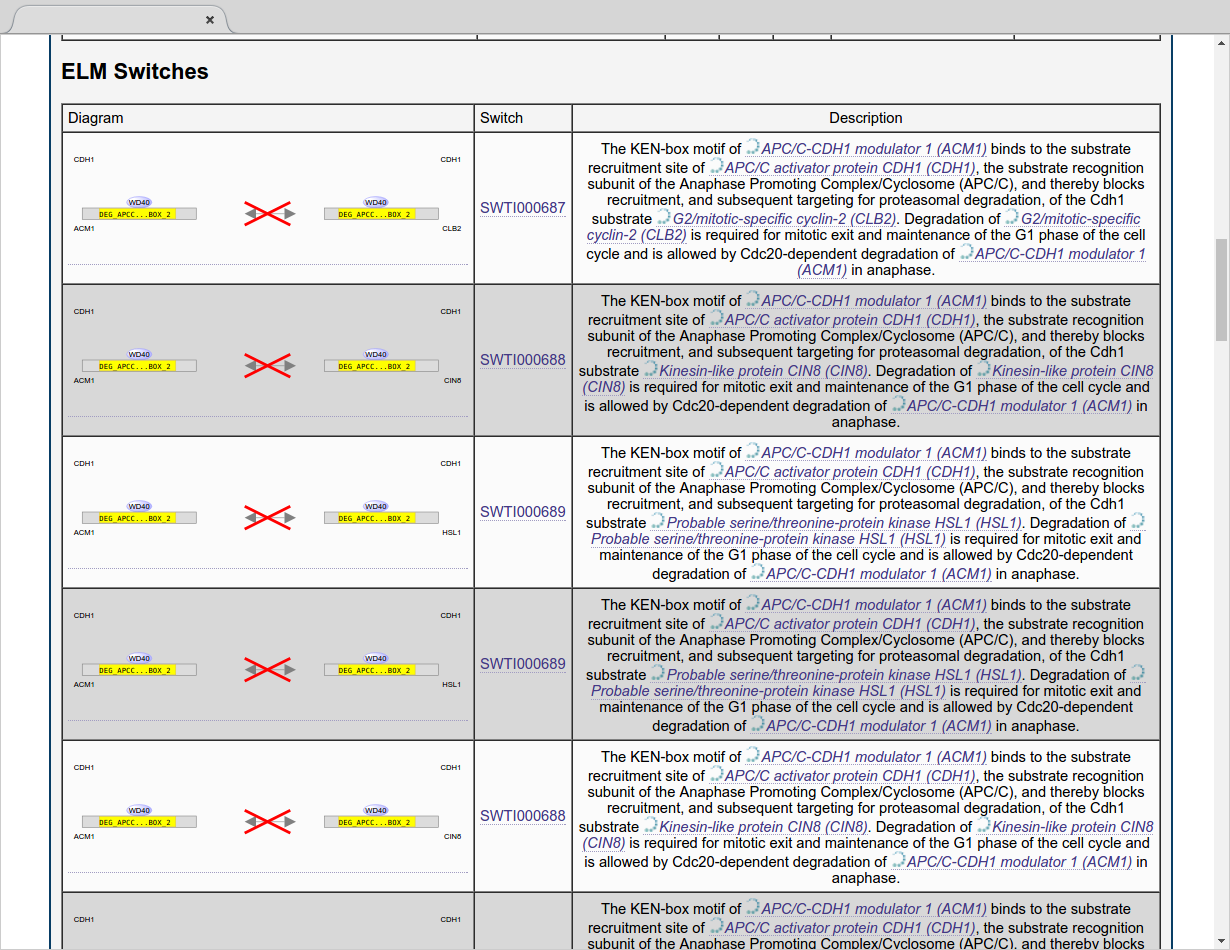
\includegraphics[width=\textwidth]{Figures/TP53_3/TP53_switches.png} 
\caption{
\textbf{Figure TP53-AP1-2}
}
\end{figure}

\begin{figure}[h!]
\centering
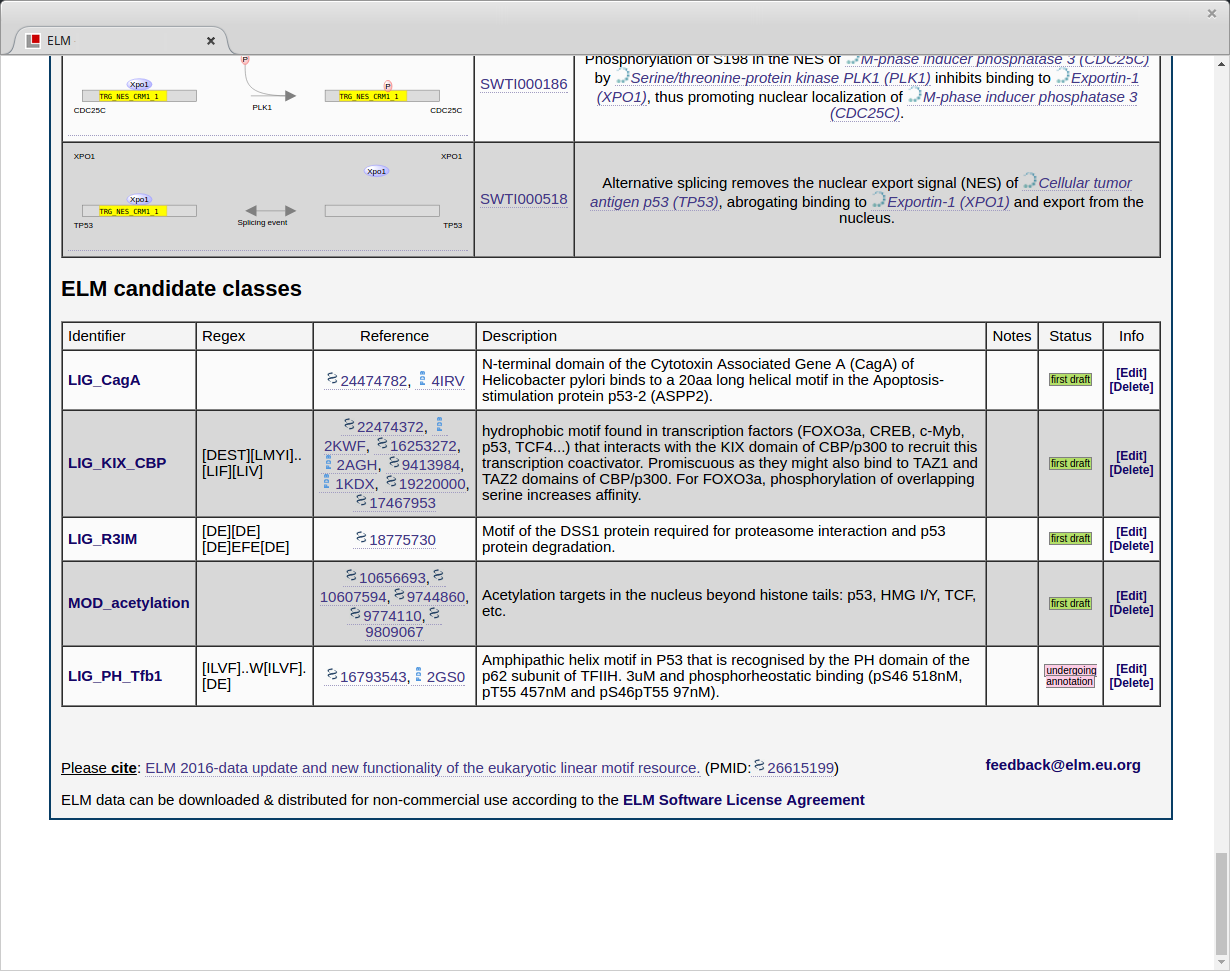
\includegraphics[width=\textwidth]{Figures/TP53_3/TP53_candidates.png} 
\caption{
\textbf{Figure TP53-AP1-3}
}
\end{figure}

Example 1: perform a search using the keyword `p53'. The results are
retrieved in the following section: ELM instances (xx matches), ELM
Switch (xx matches), and ELM Candidate classes (xx matches). One will
find proteins such as CDH1\_YEAST (because of its accession P53197)
which may or may not be what one wants.

\begin{figure}[h!]
\centering
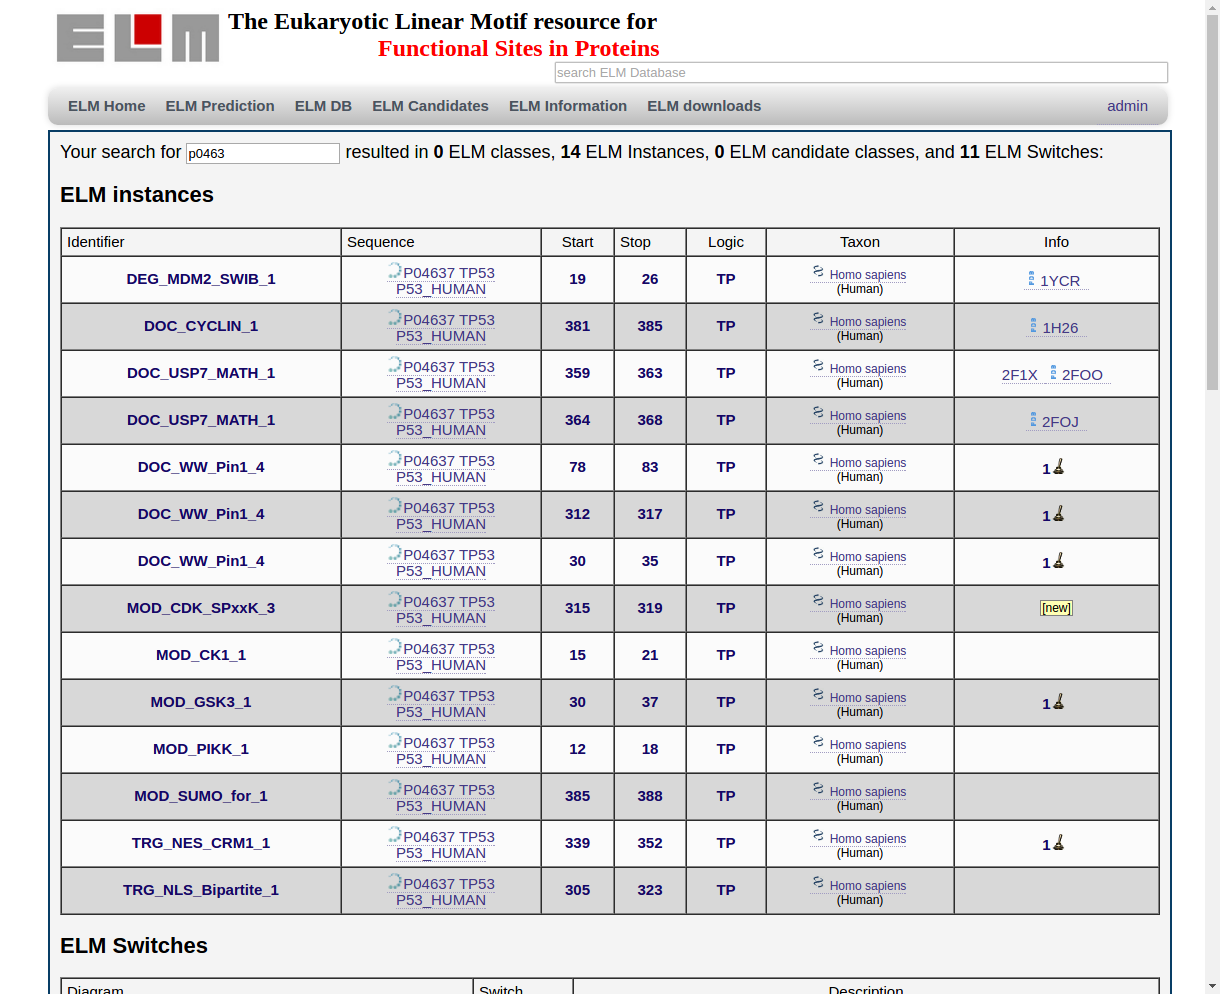
\includegraphics[width=\textwidth]{Figures/TP53_3/P04637_instances.png} 
\caption{
\textbf{Figure TP53-AP1-4}
}
\end{figure}

Example 2: perform a search using the gene id TP53 or the UniProt Acc
P04637. The results are retrieved in the following section: ELM
instances (xx matches), ELM Switch (xx matches). The retrieved hits are
less, but more specific compared with the search with `53'. However,
there are no matches in ELM Candidate classes tough some content is
related to the p53 protein.

